%_____________________________________________________________________________________________ 
% LATEX Template: Department of Comp/IT BTech Project Reports
% Main Report
% Sun Apr 1 20:40:00 IST 2011
% 
%_____________________________________________________________________________________________ 

\documentclass[a4paper,12pt,onecolumn]{report}

%_____________________________________________________________________________________________ 
% Inclusion of Required Packages
%_____________________________________________________________________________________________ 
\usepackage[dvips]{graphics}
\usepackage{color}
\usepackage{epsfig,float}
\usepackage{hyperref}
\hypersetup{
    colorlinks=true,
    linkcolor=black,
    urlcolor=cyan,
    pdfpagemode=FullScreen,
    }

%_____________________________________________________________________________________________ 
% Page Layout
%_____________________________________________________________________________________________

 \usepackage[left=2.5cm,top=2cm,right=2cm,bottom=2cm,bindingoffset=0.5cm]{geometry}

%\usepackage{geometry}
%\geometry{a4paper,left=35mm,right=20mm,top=20mm,bottom=20mm}
\setlength{\textwidth}{6.5in}
\setlength{\textheight}{10in}
\setlength{\topmargin}{0.0in}
\setlength{\oddsidemargin}{0.0in}			% Customisable
\setlength{\headheight}{0.0in}
\setlength{\headsep}{0.0in}
\setlength{\topskip}{0.0in}
%_____________________________________________________________________________________________ 
% Font Definition
%_____________________________________________________________________________________________ 
\fontencoding{T1}		% Font specification : Times New Roman, Bold, Normal, 18
\fontfamily{cmr}		% Roman
\fontseries{m}			% Medium
\fontshape{n}			% Upright
\fontsize{14pt}{5}		
\linespread{1.5}		% Vertical spacing between lines
\selectfont			% Select the specified font
%_____________________________________________________________________________________________ 
% Main report starts here
%_____________________________________________________________________________________________ 

\begin{document}	% Start of Report
%_____________________________________________________________________________________________ 
%\pagestyle{empty}
%_____________________________________________________________________________________________ 
% Title page: Specifies a custom-made title page
%_____________________________________________________________________________________________ 
\DeclareGraphicsExtensions{.png, .ps}
\begin{titlepage}
\begin{center}
\LARGE{\bf{Route Alignment using GIS, Remote Sensing and Deep Learning\\}}	% LARGE = 17.28
%\vspace{10pt}
\Large{\bf{ B. Tech. Project Mid Sem Report\\}}		% Large = 14.40
\Large{\em{Submitted by\\}}
\begin{table}[htbp]
	\begin{center}
	\begin{tabular}{ l c c l }
	\Large\bf{Apurva Deshpande} & & & \Large\bf{111903020} \\[0.3cm] 
	\Large\bf{Ashlesha Joshi} & & & \Large\bf{111903022} \\[0.3cm]
	\Large\bf{Riddhi Tharewal} & & & \Large\bf{111903068} \\
	\end{tabular}
	\end{center}
	\end{table}

%\vspace{10pt}
%names of advisors
\Large{Under the guidance of\\ }
\Large{\bf{Prof. Suraj Sawant }\\}
\Large{College of Engineering, Pune\\}
%\vspace{8pt}
% this is applicable only if you have a company based project
%\large{\bf{AND}\\}	% Case changed from full uppercase. Different from doc template. Looks better
%\vspace{10pt}
%\Large{\bf{Mr. Amit Kumar Singh}\\}
%\Large{Hindustan Naturals, Inc.\\}
%\vspace{5pt}
%coep logo added
\begin{figure}[h]
\centering

\includegraphics[width=4cm,height=4cm]{COEP_logo.jpeg}
\end{figure}


\Large{\bf{DEPARTMENT OF COMPUTER ENGINEERING AND \\INFORMATION TECHNOLOGY,\\ 
COLLEGE OF ENGINEERING, PUNE-411005}}
\vfill
\large{March 2023}
\end{center}
\end{titlepage}

%\maketitle			% *Generate* the defined title. No definition - no gereration
%_____________________________________________________________________________________________ 
% LATEX Template: Department of Comp/IT BTech Project Reports
% Certificate Page
% Sun Mar 27 10:25:35 IST 2011
% 
% Note: UK English spellings used. 
%_____________________________________________________________________________________________ 
\thispagestyle{empty}
\linespread{2}
\begin{center}			% LARGE = 18
	\Large{\bf{DEPARTMENT OF COMPUTER ENGINEERING AND\\  INFORMATION TECHNOLOGY,\\ 
	       COLLEGE OF ENGINEERING, PUNE\\}}	
\end{center}

\vspace{20pt}			% Vertical space between dept name and ``certi''

\begin{center}
	\Large{\bf{CERTIFICATE\\}}
\end{center}

\vspace{20pt}

\linespread{1.5}			% Double spacing between lines
\selectfont
\large{
Certified that this project, titled ``TITLE OF THE PROJECT''
has been successfully completed by \\ 
\begin{table}[htbp]
	\begin{center}
	\begin{tabular}{ l c c l }
	\Large\bf{ABC} & & & \Large\bf{MIS No} \\ [0.3cm]
	\Large\bf{XYZ} & & & \Large\bf{MIS No} \\ [0.3cm]
	\Large\bf{PQR} & & & \Large\bf{MIS No} \\
	\end{tabular}
	\end{center}
	\end{table} \\
and is approved for the partial fulfillment of the requirements for the degree of 
``B.Tech. Computer Engineering''.
}

\vspace{60pt}

\begin{center}		% Horizontal spacing used to keep the signatures in columns at the ends of
			% lines

SIGNATURE\hspace{\stretch{1}}SIGNATURE\\
\normalsize{\bf{NAME OF GUIDE\hspace{\stretch{1}}NAME OF HOD\\
Project Guide\hspace{\stretch{1}}Head}\\
Department of Computer Engineering\hspace{\stretch{1}}Department of Computer Engineering\\
and Information Technology,\hspace{\stretch{1}}and Information Technology,\\
College of Engineering Pune,\hspace{\stretch{1}}College of Engineering Pune,\\
Shivajinagar, Pune - 5.\hspace{\stretch{1}}Shivajinagar, Pune - 5.}
\end{center}



%_____________________________________________________________________________________________ 
% LATEX Template: Department of Comp/IT BTech Project Reports
% Abstract of Report
% Sun Mar 27 10:34:00 IST 2011
%_____________________________________________________________________________________________ 
%\newpage

%This page is to add the scanned copy of plagiarism percentage page signed by your Project Guide


\newpage
%\begin{abstract}
%\addcontentsline{toc}{chapter}{Abstract}	% This makes sure abstract is included in contents.
\begin{center}
\Large \textbf{Abstract}
\end{center}
Twas brillig and the slithy toves, Did gyre and gimball in the wabe.  All mimsy were the borogoves, And the mome-raths outgrabe. While conceding that India were the favourites to lift the World Cup on Saturday, Sri Lanka captain Kumar Sangakkara refused to term his own band of men as the underdogs in the mega event's summit clash at the Wankhede Stadium.

``They (India) are a very good side and they have always been the favourites to win this tournament. They've got to the finals and everyone will be looking for them to keep going,'' he told a media conference on the eve of the match. 
%\end{abstract}

%_____________________________________________________________________________________________ 
	% Absract: Independently typeset in file abstract.tex

\thispagestyle{empty}
\tableofcontents		% *Generate* the table of contents. No content - no table
				% LATEX needs to run 2-3 times over source to get this correct

\pagenumbering{roman}	% Lowercase roman numbering for prelim sections


\listoffigures
\addcontentsline{toc}{chapter}{List of Figures}


\newpage
\pagenumbering{arabic}	% Change to Arabic numbers for main chapters.

%_____________________________________________________________________________________________ 
% LATEX Template: Department of Comp/IT BTech Project Reports
% Sample Chapter
% Sun Mar 27 10:25:35 IST 2011
%
% Note: Itemization, enumeration and other things not shown. A sample figure is included.
%_____________________________________________________________________________________________ 

\chapter{Introduction}
\section{Jabberwock}
%Th is is a section. We can cite a reference like this: \cite{INTERNET} 	
						% Citation. See references.tex for the entry.
\subsection{Vorpal blade}
And this is a subsection.
	
\subsubsection{Tumtum tree}
You get the drift \ldots
		
\section{Jubjub Bird}

\begin{figure}[htbp]			% Sample figure 
\begin{center}
%\input{fig1.latex}			% Be sure to have the input file in the directory
\caption{A simple figure: Square}	% This will appear in the list of figures
\label{circle}
\end{center}
\end{figure}

%_____________________________________________________________________________________________ 
	% Add each chapter here in this fashion.
%_____________________________________________________________________________________________ 
% LATEX Template: Department of Comp/IT BTech Project Reports
% Sample Chapter
% Sun Mar 27 10:25:35 IST 2011
%
% Note: Itemization, enumeration and other things not shown. A sample figure is included.
%_____________________________________________________________________________________________ 

\hypersetup{
    linkcolor=blue,
}
{\let\clearpage\relax \chapter{Literature Review}}
\section{Review Process}\\The systematic review was conducted by reading research papers. In order to retrieve the papers for our systematic review, we conducted keyword searches in Google Scholar, Scopus, Science Direct, ACM, ASCE and IEEE using the terms: 
\begin{enumerate}
    \item Road Route Alignment
    \item Route Planning System
    \item Route Selection System
\end{enumerate} By reading the titles of the research papers, The papers were downloaded. As a result of the search conducted on October 23, 2022, 180 research papers were downloaded based on their titles. A total of 35 papers were selected based on the inclusion and exclusion criteria for our systematic literature review. Papers involving the use of hyperspectral images, involving language other than english or performing route selection and alignment of road networks, pipelines, railway networks were excluded from our literature review. In reviewing the full texts of the remaining relevant papers, we collected the following types of information useful for a systematic literature review: Procedure of route alignment of roads and highways, different algorithms used for route selection and alignment including - Dijkstra, A star and other shortest path algorithms; Genetic algorithms, Swarm intelligence, Fuzzy logic and other DL/ML based algorithms; details of cost functions and factors involved in route selection considering economic, social and environmental implications, and analyzing the type and features of study area using various approaches and creating corresponding maps.
\begin{figure}[H]
	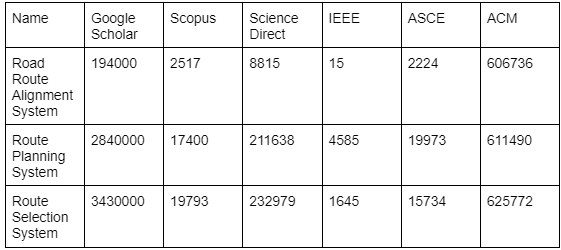
\includegraphics[width=475pt,height=275pt]{record.png}
	\caption{Total number of paper available for particular topic on particular site}
\end{figure}
\begin{figure}[H]
	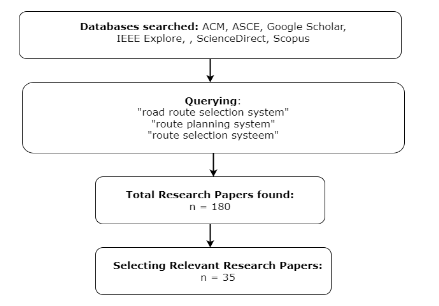
\includegraphics[width=475pt,height=325pt]{process.png}
	\caption{Process of Selection of papers for Systematic Literature Review using PRISMA analysis}
\end{figure}
\begin{figure}[H]
	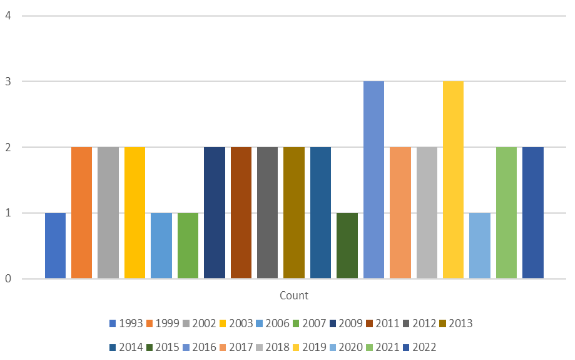
\includegraphics[width=475pt,height=275pt]{year_wise_count.png}
	\caption{Year wise count of included papers}
\end{figure}
\section{Stages involved in Route Alignment : }
\begin{figure}[H]
	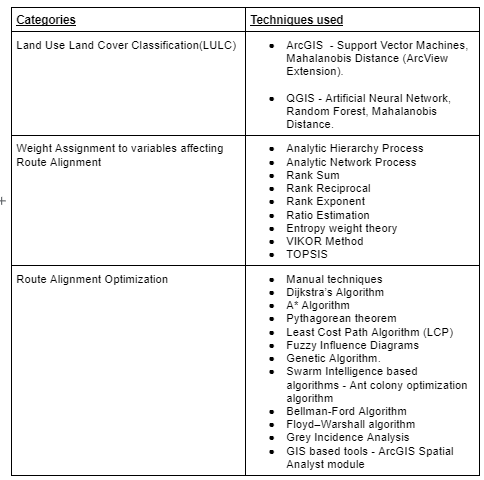
\includegraphics[width=475pt,height=425pt]{stages.png}
\end{figure}
\section{Literature Survey}
\subsection{Factors affecting route alignment : }
A correct plan for route alignment requires consideration of a number of factors or variables for construction of a function or model (\href{ https://ieeexplore.ieee.org/document/6675923}{Application of GIS in Highway Alignment with Soft Computing tools}). These factors include topography, environment, contour, geomorphology, geology, drainage, climate, cost, social, landuse and landcover.Topographic maps, aerial photographs, geological maps, soil maps, as well as various surveys can be used to analyze these factors. (\href{https://ieeexplore.ieee.org/document/8068706}{Remote Sensing and Geographical Information System Applications in Highway Alignment between the strips — Perundurai to Palani, Tamil Nadu, India}).Different types of factors can be measured via various cost functions , such as:
\begin{enumerate}
    \item Economic factors: can be calculated considering highway alignment and construction costs.
    \item Social and cultural factors: can be measured  considering accessibility cost, utility costs and proximity costs.
    \item  Environmental factors: can be estimated using Environmental Impact Assessment(EIA). It estimates the impact of route construction on the environment (soil, water, forests, climate) using penalty functions, and assigns corresponding values to alternative alignments.
\end{enumerate}

The variables are then represented in software like ArcGIS to create web maps and analyze geospatial data necessary for route alignment.The alignment plan is selected based on further studies performed with ArcGIS.
\subsection{Techniques for assigning weights to factors affecting route alignment : }
\textbf{Formal Decision Analysis : }
Formal decision analysis is used to assess the overall impact of different route alignments and decide the optimal alignments by ranking their impact on economic, social, environmental and utility factors. An initially used process from earlier times, it involved manually deciding the highway alignments, and then using decision analysis to rank them. (\href{https://ascelibrary.org/doi/10.1061/%28ASCE%290733-947X%281993%29119%3A3%28317%29 }{Decision Analysis of Alternative Highway Alignments}). Initially, the decision problem is structured by identifying the impact factors(land use, relocation, cultural & biological resources involved etc.), attributes to measure those impact factors, and selecting the alternative alignments possible by the stakeholders. Then, for every alignment, the attributes are assigned values depending on their impact  levels, and trade offs (considering penalty and cost functions).(\href{https://ascelibrary.org/doi/abs/10.1061/(ASCE)0733-947X(1999)125%3A2(144)}{GIS Platform for Multicriteria Evaluation of Route Alignments}). It is an effective process to evaluate alignments rationally and consider all multiple attributes involved in route alignment optimization but is time consuming due to manual intervention involved. Hence, further GIS tools including ArcGIS, Spatial Modules are developed to ease the process based on formal decision analysis techniques. Multi Criteria Evaluation or Multi Criteria Decision Analysis methods are also based on similar concepts, used to select important attributes or factors as per given area maps and purpose involved, which is then used to calculate the cost matrix for optimization. (\href{https://ascelibrary.org/doi/abs/10.1061/(ASCE)0733-947X(1999)125%3A2(144)}{GIS Platform for Multicriteria Evaluation of Route Alignments}). In this, various alternative attributes involved are ranked manually by the stakeholders, and the attributes are decided.(\href{https://link.springer.com/article/10.1007/s12517-017-3076-z
}{Multi-criteria GIS modeling for optimum route alignment planning in outer region of Allahabad City, India}). It is simple but less efficient, and can be optimized using different GIS tools for decision making.\\
\textbf{Weight ranking methods}
Multi-criteria weight methods are used to assign weights to input parameters/ factors affecting route alignment (as discussed in section 1). In each of the maps, the weight cost matrix is generated by weight assignment to the attributes and corresponding direction maps are plotted to visualize different factors involved in route alignment optimization. (\href{https://www.sciencedirect.com/science/article/pii/S1110982321000399}{Route alignment planning for a new highway between two cities using Geoinformatics techniques}). Five weight assignment methods are discussed as follows:
\begin{enumerate}
\item \textbf{Analytic Hierarchy Process (AHP) method - }
In this, a pairwise comparison matrix is constructed considering all input parameters. Each  attribute is given a score in the range of 10 by comparing the factors in terms of relative importance to an objective, and the resultant matrix generated is called the importance matrix. The importance matrix has the total weight of attributes, depicting its contribution towards best path identification.(Higher the weight, more important the factor).

\item \textbf{Rank Sum method - }
Rank sum is a non parametric procedure used in random sampling. 
Here, parameters involved are: 
wj is the normalized weight for the jth criteria
r is the rank position of the criterion
n is the total number of criteria under consideration

\item \textbf{Rank Reciprocal method - }
In this method, rank reciprocal weights are derived from the normalized reciprocals of a criterion’s rank.
Here, parameters involved are: 
wj is the normalized weight for the jth criteria
n is the total number of criteria under consideration 
r is the rank position of the criterion

\item \textbf{Rank Exponent method - }
In this, the decision makers initially assign weights to the most important factor/ criterion on a scale of 0-1, and then the weights of remaining factors are determined. 
Here,parameters involved are:
wj is the normalized weight for the jth criteria
r is the rank position of the criterion
n is the total number of criteria under consideration 

\item \textbf{ Ratio Estimation method - }
In this, an arbitrary weight is assigned to the most important factor on a scale of 0-100. The weights of remaining factors are estimated and smaller weights are assigned to less important factors. The procedure is continued until the weight to least important criterion is assigned. Finally, ratios of each of the factors are calculated with respect to least important factor, for relative comparison of factors involved.
\end{enumerate}
 \textbf{Entropy Weight Theory}
The concept of entropy weight theory is used to assign weights to different decision making variables involved in highway route alignment. Initially, an evaluation matrix of the route plan is created considering multiple attributes, objectives and indexes, and these are combined to generate a single synthesis index using entropy and entropy weight theory. Indexes can be classified as qualitative or quantitative, depending upon their impact and are assigned an index value using a 10 point system.Then the entropy weight decision making model is applied, which includes the following \textbf{4 steps:}
\begin{enumerate}
\item Scheme of evaluation, and indexes are decided, and a matrix is constructed considering cost and benefit of each scheme (or factor)
\item Entropy of each evaluation index is calculated as
Accordingly, the entropy weight of the index is calculated.
As per the entropy theory, a given index is a more important factor for decision making if it has smaller entropy weight and the difference of the same index for different schemes is larger.
\item Weight normalized matrix is constructed for each evaluation index, and the importance of factors are estimated using evaluation metrics such as - distance(difference between ideal point and evaluation point) and fidelity (distance of evaluation and ideal point / distance of ideal point to negative point).
\item Schemes (or factors) are selected according to their fidelity values. A scheme having smaller fidelity is considered more important for optimization. (\href{https://ascelibrary.org/doi/10.1061/41042%28349%2916}{Decision-Making Model of Highway Route Plan Based on Entropy and Entropy Weight Theory}).
\end{enumerate}
Towards the end, the best road alignment plan can be chosen by comparing synthesis index values. This decision making model is based on objective, hence the results are more realistic. Moreover, it also considers relationships between different factors involved in highway construction using their entropy, hence optimal routes can be selected.

\subsection{Techniques for Route alignment Optimization }
\textbf{Least Cost Path Algorithm (LCP)}\\Least Cost Path Algorithm is used to calculate least cost path joining start and end points for highway route alignment. With the help of the spatial analyst extension, ArcGIS software can generate the Least Cost Path Algorithm. Initially, a cost function is decided which considers the cost of construction (avoiding slopes, swampy areas), environmental area covered (water, forests etc.), social and cultural impact costs( damage to agricultural lands, moving of communities), via estimating multiple attributes involved using GIS based tools (\href{https://www.researchgate.net/publication/320005801_LEAST_COST_PATH_ALGORITHM_DESIGN_FOR_HIGHWAY_ROUTE_SELECTION}{Least Cost Path Algorithm Design for Highway Route Selection}). Once the cost parameters are decided, LCPA uses the cost-weighted distance and the direction surfaces for an area to determine a cost-effective route between a source and a destination location. The process is repeated until the source and destination points are connected via route having minimal cost. LCP analysis is used for optimizing social, environmental, economical, and technical aspects of the route alignment and can also be implemented effectively using GIS based tools as well (\href{https://link.springer.com/article/10.1007/s12517-017-3076-z}{ Multi-criteria GIS modeling for optimum route alignment planning in outer region of Allahabad City}).\\
\textbf{Fuzzy Logic}
Fuzzy logic refers to many-valued logic, in which the truth values of variables may be any real number between 0 and 1.A fuzzy logic approach can be useful when route alignment is being considered, since the results are not always accurate for any particular plan of route alignment.(\href{https://ieeexplore.ieee.org/document/6675923
}{Application of GIS in Highway Alignment with Soft Computing tools}). Fuzzy logic has also found applications in influence diagrams which can be used for constructing route alignment models. Using a fuzzy influence diagram, a model can be constructed to characterize the risk of a route alignment plan and to make a risk-based decision (\href{https://ieeexplore.ieee.org/document/6414422}{Research on Highway Alignment Decision-making based on complex system risk analysis}). It is advantage to use fuzzy logic when precise inputs are not required. \\
\textbf{Genetic algorithms and Swarm Intelligence}
Genetic algorithm is used for both constrained and unconstrained optimization that is inspired by natural selection, a process that drives biological evolution. GAs were first utilized for highway alignment optimization by Jong (1998). (\href{https://ascelibrary.org/doi/10.1061/40652%282003%297}{Optimizing Highway Networks- A Genetic Algorithms and Swarm Intelligence Based Approach})It uses the principle of orthogonal cutting planes,in which the straight line joining start and end points is divided into intervals(number of intervals decides the precision of optimization) (Diag. Pg 3), and each plane passes through an interval. It further states that the optimal highway alignment will always cross through exactly one point lying along each plane(formed passing through each interval of lines . 
There are \textbf{3 steps} involved in route optimization using Genetic algorithms : 
\begin{enumerate}
\item Genetic encoding and initial population is decided: For alignment of n intersection points in the intervals, the encoded solution has 2n genes. Hence, genes in chromosome and coordinates of intersection points are mapped ( as : (lambda)2i-1 = di … for all i = 1, 2, … n)
\item Genetic operators are applied to solved the optimization problem - it includes mutation based and crossover based operators - designed to work on the decoded intersection points
\item Optimal search is performed - Initially, the initial population is generated, and further generations, better solutions are searched by applying the genetic algorithm to minimize the objective function/ cost function. Cost function is decided considering the length dependent costs (construction, maintenance) and location dependent (right of way) costs. This step is used to produce optimized route alignments, to connect the start and end points by curve fitting.
\end{enumerate}
It takes longer time to search optimized route(s) using GAs, and the variation in cost functions reduce towards successive generations
GA can be further optimized by using swarm intelligence algorithm, which is inspired by the collective behavior of social insect colonies. It decides the evolution of genes in further generations, by selecting the intermediate planes for optimal search randomly. Hence, using SI with GA, reduces the computational efficiency and reaches optimal path quicker, although it is harder to apply SI for route optimization in regions with greater land variability, and route network optimization. (\href{https://www.sciencedirect.com/science/article/pii/S0968090X11001422}{Applicability of highway alignment optimization models}). To determine the optimum horizontal highway alignment using station points, an integrated GIS-GA model has also been developed.
\subsection{Other Techniques }
Hand drawn alignment sketches are also being used. In one study, hand-drawn alignment sketches on maps were easily converted into vector drawings, and all alignment coordinates and element data were stored in a data bank.Based on different criteria, the evaluation module for the generated vector representation of alignments is called a cost model (GMAPS-GCARS), which is actually formed by joining the nodes of a cost-model matrix, where each node is assigned a cost of traversing it - using the Dijkstra algorithm and Genetic Algorithm. Dijkstra's algorithm is commonly used for optimizing route alignments and finding shortest routes in many studies (\href{https://ascelibrary.org/doi/10.1061/40630%28255%29172 }{Interactive and Graphic Systems for Highway Location and Route Selection}).
\subsection{GIS tools for Route Alignment}
The alignment of routes has also been accomplished through the use of a variety of tools. ArcGIS, ArcInfo and ArcView are primarily used to digitize the land use, road networks and other variables within the given area. In these tools, initially the satellite images obtained are converted to vector layers. Then the layers are stacked onto each other, to obtain different cost criterion maps for land use/land cover, physical features, slope, forest, water areas, which are further converted to raster form and used to calculate cost matrix involved in alignment optimization. A Quantm computer-based planning tool was utilized for alignment optimization, which is capable of performing cost-based alignment optimization, generating low cost road or railway alignments automatically (\href{https://doi.org/10.1016/S0968-090X(00)00040-1}{New Technologies for Transport Route Selection}). As an alternative to a single least cost path, it provides a set of alternatives that take into consideration different social and economic factors and allow people to select their preferred alignment, resulting in lower costs. 
ArcGIS provides various tools for route alignment optimization, some of the tools used for route alignment include:
\begin{enumerate}
\item \textbf{Weighted Overlay Analysis (WOA) tool}: used for surface cost analysis to find out important factors involved in cost estimation using multi criteria evaluation/ multi attribute decision making. (\href{https://link.springer.com/article/10.1007/s12517-017-3076-z}{Multi-criteria GIS Modeling for Optimum Route Alignment Planning in Outer Region of Allahabad City}).
\item \textbf{Spatial Module}: used to perform alignment optimization by minimizing cost of path from source to destination.
\item \textbf{Polyline feature conversion tools}: used to convert optimum route alignment(s) calculated in raster form to polyline features for better visualization of path(s).
\end{enumerate}
GIS based tools can be utilized to perform overlays of maps, create buffers and rasters, analyze datasets of images through visualization, and cost optimization using various techniques.It provides a simple and efficient way to implement route alignment optimization through different modules available.



%_____________________________________________________________________________________________ 

%_____________________________________________________________________________________________ 
% LATEX Template: Department of Comp/IT BTech Project Reports
% Sample Chapter
% Sun Mar 27 10:25:35 IST 2011
%
% Note: Itemization, enumeration and other things not shown. A sample figure is included.
%_____________________________________________________________________________________________ 

\chapter{Research Gaps and Problem Statement}
\section{Research Gaps: }
\text{The established techniques used for route alignment of roads and highways currently involve surveying the roads and deciding the alignments considering the economical costs (earthwork costs, construction costs, labor and material costs etc.) and utility costs (traffic costs, costs of construction over railway and river crossings etc.). The process of surveying and getting information of the factors involved is done manually by the stakeholders, and then the optimal highway alignments are decided either manually or by using GIS tools. This process is often time consuming, and may involve human errors in deciding the optimal alignments which might lead to economical, social and environmental losses in the future.}\newline
\text{Hence, this is a research gap we aim to solve, by considering all the factors involved in road construction and alignment using a multi-criteria decision making process including economical, social, cultural, utility and environmental factors and ranking them according to their importance for road alignment using weight assignment and ranking techniques. Finally, the optimized route alignment can be decided considering all the costs involved, using machine learning and route optimization techniques. This process is more efficient and accurate to predict optimized alignments for roadways.}\newline
\text{Furthermore, the current methods for performing route alignment using softwares like ArcGIS or QGIS, do not consider environmental and social factors getting affected by road construction considerably. This involves environmental factors - rivers and water bodies, forest resources, soil and drainage systems; and social factors - communities getting affected by highway construction, traffic involved after construction etc.. We aim to solve this research gap by considering multi objective based route alignment optimization specifically considering environmental factors as well as other important factors added as separate layers in cost optimization. This problem can be solved efficiently using current deep learning and machine learning based models for optimization with better accuracy.}\newline
\text{Additionally, we aim to utilize and compare established techniques used for LULC classification, Multi criteria Decision Making, Weight Ranking and Route Optimization reviewed in section [2] with recently developed techniques involving machine learning and deep learning based classifiers and optimizers, as well as automated ranking methods for factors involved in road construction, to thoroughly research the techniques for route alignment optimization for better accuracy, lesser time and space complexity.}\newline

\section{Problem Statement: }
\text{After performing the literature review and understanding the research gaps involved in existing techniques used in road alignment, our research project solve the \textbf{Problem Statement: To improve route alignment optimization using deep learning and machine learning based models considering all the factors involved as per their importance, for better accuracy and time complexity}.}\newline
\section{Research Objectives:}
\begin{enumerate}
    \item To utilize recently developed deep learning based models, along with existing techniques for LULC classification to understand resources involved in a region - land utilization, slope and aspect of land involved, soil, forest, water etc. using satellite images
   \item  To implement multi criteria decision making and weight ranking techniques to decide importance of factors involved in route alignment and perform route optimization considering the economical, social and environmental factors using current machine learning and deep learning based models as well as existing techniques for multi-objective optimization
   \item To research and compare different techniques for route alignment optimization based on their accuracy, time and space complexity
   \item  To predict optimized route alignments for the decided study area (Pune-Mumbai highway) using GIS, DL and ML based techniques by minimizing the costs involved as well as minimizing the social and environmental impacts of highway construction.

\end{enumerate}
% %Th is is a section. We can cite a reference like this: \cite{INTERNET} 	
% 						% Citation. See references.tex for the entry.
% \subsection{Vorpal blade}
% And this is a subsection.
	
% \subsubsection{Tumtum tree}
% You get the drift \ldots
		
% \section{Jubjub Bird}

% \begin{figure}[htbp]			% Sample figure 
% \begin{center}
% %\input{fig1.latex}			% Be sure to have the input file in the directory
% \caption{A simple figure: Square}	% This will appear in the list of figures
% \label{circle}
% \end{center}
% \end{figure}

%_____________________________________________________________________________________________ 

%_____________________________________________________________________________________________ 
% LATEX Template: Department of Comp/IT BTech Project Reports
% Sample Chapter
% Sun Mar 27 10:25:35 IST 2011
%
% Note: Itemization, enumeration and other things not shown. A sample figure is included.
%_____________________________________________________________________________________________ 

\chapter{Proposed Methodology/ Solution}
\section{Jabberwock}
%Th is is a section. We can cite a reference like this: \cite{INTERNET} 	
						% Citation. See references.tex for the entry.
\subsection{Vorpal blade}
And this is a subsection.
	
\subsubsection{Tumtum tree}
You get the drift \ldots
		
\section{Jubjub Bird}

\begin{figure}[htbp]			% Sample figure 
\begin{center}
%\input{fig1.latex}			% Be sure to have the input file in the directory
\caption{A simple figure: Square}	% This will appear in the list of figures
\label{circle}
\end{center}
\end{figure}

%_____________________________________________________________________________________________ 

%_____________________________________________________________________________________________ 
% LATEX Template: Department of Comp/IT BTech Project Reports
% Sample Chapter
% Sun Mar 27 10:25:35 IST 2011
%
% Note: Itemization, enumeration and other things not shown. A sample figure is included.
%_____________________________________________________________________________________________ 

\chapter{Experimental Setup}
\section{Jabberwock}
%Th is is a section. We can cite a reference like this: \cite{INTERNET} 	
						% Citation. See references.tex for the entry.
\subsection{Vorpal blade}
And this is a subsection.
	
\subsubsection{Tumtum tree}
You get the drift \ldots
		
\section{Jubjub Bird}

\begin{figure}[htbp]			% Sample figure 
\begin{center}
%\input{fig1.latex}			% Be sure to have the input file in the directory
\caption{A simple figure: Square}	% This will appear in the list of figures
\label{circle}
\end{center}
\end{figure}

%_____________________________________________________________________________________________ 

%_____________________________________________________________________________________________ 
% LATEX Template: Department of Comp/IT BTech Project Reports
% Sample Chapter
% Sun Mar 27 10:25:35 IST 2011
%
% Note: Itemization, enumeration and other things not shown. A sample figure is included.
%_____________________________________________________________________________________________ 

\chapter{Results and Discussion}
\section{Results}
This paper discuss different algorithm and strategies used to optimize route alignment till date. The base-case scenario involves optimizing the highway alignment
based on different factors to minimize cost and maximize profit.
LULC will be performed which will classify the regions of the input map into soil, forest, water, etc classes to determine the parameters involved. AHP is the most accurate technique for weight assignment and ranking of factors based on our review. Genetic algorithms, used with Swarm intelligence predicts the optimal routes faster, taking less time and space complexity based on current literature survey. Thus considering study area as Pune-Mumbai region, our project aims to align the route optimally which will reduce total travel time and traffic, as well as minimize cost and adverse effects of highway construction. We aim to further use current DL and ML based models to increase efficiency and accuracy of route alignment further.
\section{Challenges and Future Directions}
In the process of route alignment, route optimization is a crucial step. The genetic algorithm is the most commonly used algorithm in this step. It has many advantages but also faces some challenges like selection of initial population, efficient fitness functions, encoding schemes, premature convergence and degree of mutation/crossover. A fuzzy logic system should ensure that the rules are not flawed in order to ensure that the results are accurate.The other algorithms listed for route alignment optimization will assist in reaching better accuracy and expanding the application of computer science in route alignment. 
\newline
In route alignment, we can either consider a single factor as a whole or assign weight to each entity in consideration and then using some function calculating cumulative weight, these can provide an optimal path in return. One of the major problems in assigning weight is the determination of the relative importance of one parameter with respect to the other. Thus weight assignment can be done depending on their importance to route alignment requirements.


\begin{figure}[htbp]			% Sample figure 
\begin{center}
%\input{fig1.latex}			% Be sure to have the input file in the directory
	% This will appear in the list of figures
\label{circle}
\end{center}
\end{figure}

%_____________________________________________________________________________________________ 

%_____________________________________________________________________________________________ 
% LATEX Template: Department of Comp/IT BTech Project Reports
% Sample Chapter
% Sun Mar 27 10:25:35 IST 2011
%
% Note: Itemization, enumeration and other things not shown. A sample figure is included.
%_____________________________________________________________________________________________ 

\chapter{Conclusion}
The goal is to develop an optimal route alignment between Pune and Mumbai. As part of the process, three stages will be completed: Land Use and Land Cover Classification (LULC), Weight Assignment and Ranking of Factors, and Route Alignment Optimization, and the most effective results from each stage will be considered for further processing. We are thus currently working on LULC using Python and its libraries to understand the landscape of the study area. The challenge is to develop and test the model on a large dataset. After completion of LULC, we will use the suitable weight ranking method for assigning weights to different factors affecting route alignment. As a final step ,we will work on optimizing the route. The final route alignment will thus be safe, economical, and optimal. Additionally, in order to examine approaches, applications, and trends in Deep Learning, Machine Learning, GIS and Remote Sensing in the field of Route Alignment, we have conducted a comprehensive study and documented it in the form of a review paper. 

\begin{figure}[htbp]			% Sample figure 
\begin{center}
%\input{fig1.latex}			% Be sure to have the input file in the directory	% This will appear in the list of figures
\label{circle}
\end{center}
\end{figure}

%_____________________________________________________________________________________________ 

%_____________________________________________________________________________________________ 
% LATEX Template: Department of Comp/IT BTech Project Reports
% Sample Chapter
% Sun Mar 27 10:25:35 IST 2011
%
% Note: Itemization, enumeration and other things not shown. A sample table is included.
%_____________________________________________________________________________________________ 
% \documentclass{article}
% \usepackage{enumitem}% http://ctan.org/pkg/enumitem


\chapter{Bibliography}
\begin{enumerate}
  \item Bin YANG, Xiu-mei GU, Zheng-wei HE, Qing WANG, 2011, Research on geo-hazard appraisal and decision in highway based on GIS Technology, \url{https://ieeexplore.ieee.org/document/5982236}
\item Chan Weng Tat, Fan Tao, 2003, Using GIS and genetic algorithm in highway alignment optimization, \url{https://ieeexplore.ieee.org/document/1252747}
\item S. Loganathan, K. Elangovan, 2013, Application of GIS in highway alignment with soft computing tools, \url{https://ieeexplore.ieee.org/document/6675923}
\item S. Loganathan, K. Elangovan, 2017, Remote sensing and geographical information system applications in highway alignment between the strips — Perundurai to Palani, Tamil Nadu, India, \url{https://ieeexplore.ieee.org/document/8068706}
\item Wrya H. Nadir, 2021, GIS Aided Corridor Approach for Horizontal Highway Alignment Development Using GA, \url{https://ieeexplore.ieee.org/document/9476115}
\item Yan Sun, Yi Wu, Zheng Sun, 2007, Optimal Route Selection Method Based on Grey Incidence Analysis, \url{https://ieeexplore.ieee.org/document/4338998}
\item Zhichao Song, Hong Duan, Siyang Zhou, Xiaogang Qiu, 2016, Urban route planning considering traffic flows, \url{https://ieeexplore.ieee.org/document/7382822}
\item Zhi Zhou, Xin-yuan Cui, Jing-ting Wang, 2013, Research on highway alignment decision-making based on complex system risk analysis, \url{https://ieeexplore.ieee.org/document/6414422}
\item Avijit Majia, Manoj K Jha, 2011, A Multiobjective Analysis of Impacted Area of Environmentally Preserved Land and Alignment Cost for Sustainable Highway Infrastructure Design, \url{https://www.sciencedirect.com/science/article/pii/S1877042811014856} 
\item Chi Zhang, Xiao-Min Yan, Xing Huang, Tian-Yu Zhang and Wen-Jun Zhu, 2018, A Multi-Layer Evolution Algorithm for Optimizing Highway Alignments, \url{https://ascelibrary.org/doi/10.1061/9780784480915.430 }
\item D. Hirpa , W. Hare Y. , Lucet Y. , Pushak , S. Tesfamariam, 2016, A bi-objective optimization framework for three-dimensional road alignment design, \url{https://www.sciencedirect.com/science/article/abs/pii/S0968090X16000358}
\item George Triebel, P.E., M.ASCE and Todd Crouthamel, 2019, Route Selection Based on a Weighted Ranking Analysis, \url{https://ascelibrary.org/doi/10.1061/9780784482483.029}
\item Jerome L. Catbagan I and Jose Regin F. Regidor, Dr. Eng. , 2002, Interactive and Graphic Systems for Highway Location and Route Selection, \url{https://ascelibrary.org/doi/10.1061/40630%28255%291720}
\item M. Surabuddin Mondal , Rahul Dev Garg , Varun Pandey , Martin Kappas, 2021, Route alignment planning for a new highway between two cities using Geoinformatics techniques, \url{https://www.sciencedirect.com/science/article/pii/S1110982321000399 }
\item Manoj K Jha, 2003, Optimizing Highway Networks- A Genetic Algorithms and Swarm Intelligence Based Approach, 
\url {https://ascelibrary.org/doi/10.1061/40652%282003%297 }
\item Manoj K. Jha, P.E., Eungcheol Kim, 2006, Highway Route Optimization Based on Accessibility Proximity and Land Use Changes, \url{https://ascelibrary.org/doi/10.1061/%28ASCE%290733-947X%282006%29132%3A5%28435%29 }
\item Min-Wook Kang , Manoj K. Jha , Paul Schonfeld, 2012, Applicability of highway alignment optimization models, \url{https://www.sciencedirect.com/science/article/abs/pii/S0968090X11001422 }
\item Ram B. Kulkarni, Robert L. Burns, John Wright, Bryan Apper, Thomas O. Baily, s and Stephen T. Noack, 1993, Decision Analysis of Alternative Highway Alignments, \url{https://ascelibrary.org/doi/10.1061/%28ASCE%290733-947X%281993%29119%3A3%28317%29 } 
\item Saad Aljadhai and Dulcy M. Abraham, 2016, Evaluation of Proposed Highway Routes Based on the Existing Utilities- A Cost Estimate Framework, \url{https://ascelibrary.org/doi/10.1061/9780784479827.205}
\item Sabyasachee Mishra, Min-Wook Kang, M.ASCE and Manoj K. Jha, 2014, Empirical Model with Environment Considerations in Highway Route Optimization \url{https://ascelibrary.org/doi/10.1061/%28ASCE%29IS.1943-555X.0000194}
\item Zhang Yingxue, Chunhua Han and Zhang Qisen, 2009,Decision-Making Model of Highway Route Plan Based on Entropy and Entropy Weight Theory, \url{https://ascelibrary.org/doi/10.1061/41042%28349%2916}
\item Salah Sadek, Mounia Bedran and Isam Kaysi, 1999, GIS Platform for Multicriteria Evaluation of Route Alignments, \url{https://ascelibrary.org/doi/abs/10.1061/(ASCE)0733-947X(1999)125%3A2(144)}
\item T.Subramani,D.Pari, 2015, Highway Alignment Using Geographical Information System, \url{http://iosrjen.org/Papers/vol5_issue5%20(part-3)/E05533242.pdf}
\item Milan Sekulic, 2019, Multi-Criteria GIS modeling for optimal alignment of roadway 
by-passes in the Tlokweng Planning Area, Botswana, \url{https://lup.lub.lu.se/student-papers/record/8979335/file/8979344.pdf}
\item Ashok Poudel ,Pradeep Kumar Shrestha, 2022, GIS Modelling for Optimal Alignment Selection: A Case Study of Karputar to Yamdi Section, Midhill Highway, \url{http://conference.ioe.edu.np/ioegc11/papers/ioegc-11-014-11030.pdf}
\item Wojciech Chmiel, Iwona Skalna, Stanisław Jedrusik, 2018, Intelligent route planning system based on interval computing, \url{https://doi.org/10.1007/s11042-018-6714-x}
\item Duy Nguyen Duc , Thong Tran Huu and Narameth Nananukul, 2020, A Dynamic Route-Planning System Based on Industry 4.0 Technology,\url{https://www.mdpi.com/901798}
\item Ibrahim, N.; Hassan, F. H, Ab Wahab, M. N. & Letchmunan, S., 2022, Emergency Route Planning with the Shortest Path Methods: Static and
Dynamic Obstacles, \url{http://www.ijsimm.com/Full_Papers/Fulltext2022/text21-3_608.pdf}
\item Mukund Pratap Singh & Pitam Singh, 2017, Multi-criteria GIS modeling for optimum route alignment planning in outer region of Allahabad City, India, \url{https://link.springer.com/article/10.1007/s12517-017-3076-z}
\item T.Subramani, S.Nanda Kumar, 2012, National Highway Alignment Using Gis, \url{https://citeseerx.ist.psu.edu/document?repid=rep1&type=pdf&doi=088afefad15520e44a0bb6458c061fdbcc9dd2d4}
\item Debashis Das, Anil Ojha, Harlin Kramsapi, Partha P. Baruah, Mrinal Kr. Dutta1, 2019, Road network analysis of Guwahati city using GIS, \url{https://doi.org/10.1007/s42452-019-0907-4}
\item Katherine Hon, 1999, Integrating Environment Criteria in Alignment Selection, \url{https://ascelibrary.org/doi/abs/10.1061/40430%281999%2984 }
\item T. F. Fwa, W. T. Chan, Y. P. Sim, 2002, Optimal Vertical Alignment Analysis for Highway Design, \url{https://ascelibrary.org/doi/abs/10.1061/%28ASCE%290733-947X%282002%29128%3A5%28395%29}
\item Kun Miao, Liang Li, Xiao-Li Yang, Yuan-Yuan Huo, 2009, Ant Colony Optimization Algorithm for Vertical Alignment of Highways, \url{https://ascelibrary.org/doi/10.1061/41041%28348%2915}
\item Sabyasachee Mishra, Min-Wook Kang, Manoj K. Jha, 2014, Empirical Model with Environment Considerations in Highway Route Optimization, \url{https://ascelibrary.org/doi/10.1061/%28ASCE%29IS.1943-555X.0000194 }
\end{enumerate}
% This section has a sample table. 


% More signs of serious radiation contamination in and near the Fukushima Daiichi nuclear power plant were detected Thursday, with the latest data finding groundwater containing radioactive iodine 10,000 times the legal threshold and the concentration of radioactive iodine-131 in nearby seawater rising to the highest level yet.


% \begin{table}[H]		% Table
% \begin{center}		
% \begin{tabular}{ | c | c | }	% Format	
% \hline
% \multicolumn{2}{|c|}{Table 1: Test Century Records }\\
% \hline
% \bf{Batsman} & \bf{Test Centuries}\\ \hline
% Sachin & 51 \\ \hline
% Kallis & 40 \\ \hline
% Ponting & 39 \\ \hline
% Lara, Gavaskar & 34\\ 
% \hline
% \end{tabular}
% \caption{A simple table: Test centuries}	% This will appear in List of Tables
% \label{table1}
% \end{center}
% \end{table}

% Radioactive material was confirmed from groundwater for the first time since the March 11 quake and tsunami hit the nuclear power plant on the Pacific coast, knocking out the reactors' key cooling functions. An official of the plant operator Tokyo Electric Power Co. said, ''We're aware this is an extremely high figure.''

% The contaminated groundwater was found from around the No. 1 reactor's turbine building, although the radiation level of groundwater is usually so low that it cannot be measured.

% Japanese authorities were also urged to consider taking action over radioactive contamination outside the 20-kilometer evacuation zone around the plant, as the International Atomic Energy Agency said readings from soil samples collected in the village of Iitate, about 40 km from the plant, exceeded its criteria for evacuation.

% OKYO - Japan on Monday expanded the evacuation zone around its crippled nuclear plant because of high levels of accumulated radiation, as a strong aftershock rattled the area one month after a quake and tsunami sparked the worst nuclear crisis since Chernobyl.

% A magnitude 6.6 tremor shook buildings in Tokyo and a wide swathe of eastern Japan on Monday evening, knocking out power to 220,000 households and causing a halt to water pumping to cool three damaged reactors at Fukushima.

% The epicentre of the latest quake was 88 km (56 miles) east of the plant and stopped power supply for pumping water to cool reactors No. 1, No. 2 and No. 3.

% The aftershock also forced engineers to postpone plans to remove highly contaminated water from a trench at reactor No. 2.

% The government announced earlier that because of accumulated radiation contamination, it would encourage people to leave certain areas beyond its 20 km (12 mile) exclusion zone around the plant.

% Children, pregnant women, and hospitalized patients should stay out of some areas 20-30 km from the nuclear complex, Chief Cabinet Secretary Yukio Edano told reporters.

% "These new evacuation plans are meant to ensure safety against risks of living there for half a year or one year," he said. There was no need to evacuate immediately, he added.

% The move comes amid international concern over radiation spreading from the six damaged reactors at Fukushima, which engineers are still struggling to bring under control after they were wrecked by the 15-metre tsunami on March 11.

% TEPCO President Masataka Shimizu visited the area on Monday for the first time the disaster. He had all but vanished from public view apart from a brief apology shortly after the crisis began and has spent some of the time since in hospital.

% "I would like to deeply apologize again for causing physical and psychological hardships to people of Fukushima prefecture and near the nuclear plant," said a grim-faced Shimizu.

% Dressed in a blue work jacket, he bowed his head for a moment of silence with other TEPCO officials at 2:46 p.m. (0546 GMT), exactly a month after the earthquake hit.

% Fukushima Governor Yuhei Sato refused to meet him, but the TEPCO boss left a business card at the government office.

% Engineers at the damaged Daiichi plant north of Tokyo said they were no closer to restoring the plant's cooling system which is critical to bring down the temperature of overheated fuel rods and to bringing the six reactors under control.
% %_____________________________________________________________________________________________ 


				% No need to write all font and page specs in the chapter
				% files. There only typesetting tags are required.
%%_____________________________________________________________________________________________ 
% LATEX Template: Department of Comp/IT BTech Project Reports
% Sample Chapter
% Sun Mar 27 10:25:35 IST 2011
%
% Note: Itemization, enumeration and other things not shown. A sample table is included.
%_____________________________________________________________________________________________ 

\chapter{Literature Survey}
\section{Section m}
This section has a sample table. 


More signs of serious radiation contamination in and near the Fukushima Daiichi nuclear power plant were detected Thursday, with the latest data finding groundwater containing radioactive iodine 10,000 times the legal threshold and the concentration of radioactive iodine-131 in nearby seawater rising to the highest level yet.


\begin{table}[H]		% Table
\begin{center}		
\begin{tabular}{ | c | c | }	% Format	
\hline
\multicolumn{2}{|c|}{Table 1: Test Century Records }\\
\hline
\bf{Batsman} & \bf{Test Centuries}\\ \hline
Sachin & 51 \\ \hline
Kallis & 40 \\ \hline
Ponting & 39 \\ \hline
Lara, Gavaskar & 34\\ 
\hline
\end{tabular}
\caption{A simple table: Test centuries}	% This will appear in List of Tables
\label{table1}
\end{center}
\end{table}

Radioactive material was confirmed from groundwater for the first time since the March 11 quake and tsunami hit the nuclear power plant on the Pacific coast, knocking out the reactors' key cooling functions. An official of the plant operator Tokyo Electric Power Co. said, ''We're aware this is an extremely high figure.''

The contaminated groundwater was found from around the No. 1 reactor's turbine building, although the radiation level of groundwater is usually so low that it cannot be measured.

Japanese authorities were also urged to consider taking action over radioactive contamination outside the 20-kilometer evacuation zone around the plant, as the International Atomic Energy Agency said readings from soil samples collected in the village of Iitate, about 40 km from the plant, exceeded its criteria for evacuation.

OKYO - Japan on Monday expanded the evacuation zone around its crippled nuclear plant because of high levels of accumulated radiation, as a strong aftershock rattled the area one month after a quake and tsunami sparked the worst nuclear crisis since Chernobyl.

A magnitude 6.6 tremor shook buildings in Tokyo and a wide swathe of eastern Japan on Monday evening, knocking out power to 220,000 households and causing a halt to water pumping to cool three damaged reactors at Fukushima.

The epicentre of the latest quake was 88 km (56 miles) east of the plant and stopped power supply for pumping water to cool reactors No. 1, No. 2 and No. 3.

The aftershock also forced engineers to postpone plans to remove highly contaminated water from a trench at reactor No. 2.

The government announced earlier that because of accumulated radiation contamination, it would encourage people to leave certain areas beyond its 20 km (12 mile) exclusion zone around the plant.

Children, pregnant women, and hospitalized patients should stay out of some areas 20-30 km from the nuclear complex, Chief Cabinet Secretary Yukio Edano told reporters.

"These new evacuation plans are meant to ensure safety against risks of living there for half a year or one year," he said. There was no need to evacuate immediately, he added.

The move comes amid international concern over radiation spreading from the six damaged reactors at Fukushima, which engineers are still struggling to bring under control after they were wrecked by the 15-metre tsunami on March 11.

TEPCO President Masataka Shimizu visited the area on Monday for the first time the disaster. He had all but vanished from public view apart from a brief apology shortly after the crisis began and has spent some of the time since in hospital.

"I would like to deeply apologize again for causing physical and psychological hardships to people of Fukushima prefecture and near the nuclear plant," said a grim-faced Shimizu.

Dressed in a blue work jacket, he bowed his head for a moment of silence with other TEPCO officials at 2:46 p.m. (0546 GMT), exactly a month after the earthquake hit.

Fukushima Governor Yuhei Sato refused to meet him, but the TEPCO boss left a business card at the government office.

Engineers at the damaged Daiichi plant north of Tokyo said they were no closer to restoring the plant's cooling system which is critical to bring down the temperature of overheated fuel rods and to bringing the six reactors under control.
%_____________________________________________________________________________________________ 

		


\bibliographystyle{plain}  % You can change the style of writing bibliography.
\bibliography{coep_compit_report} % Instead of a .bib file, you can just write it in 
				  % a text file with \bibitem entries.
%_____________________________________________________________________________________________ 
\end{document}			% End of Report

